\documentclass[11pt,twocolumn,a4paper]{article}
\usepackage[utf8]{inputenc}\usepackage[T1]{fontenc}\usepackage[margin=2.0cm,columnsep=0.6cm]{geometry}
\usepackage{booktabs,array,hyperref,times,microtype,graphicx}
\usepackage[font=small,labelfont=bf]{caption}
\hypersetup{colorlinks=true,linkcolor=black,urlcolor=blue}
\setlength{\parskip}{4pt}
\title{\vspace{-1.2cm}\large\textbf{Puntos autom\'aticos DINOv3 para SAM~2.1 en segmentaci\'on de agua superficial Sentinel-2 (Sen1Floods11): informe E3}}
\author{\small E.~Villarreal$^{1}$ y R.~Ch\'avez$^{1}$ \\ \footnotesize $^{1}$PUCP, Ingenier\'ia Inform\'atica, Deep Learning 1INF52 (2026-2) \\ \footnotesize Repositorio: github.com/roberto-chavez/auto-prompt-sam2}
\date{\vspace{-0.6cm}\footnotesize Versi\'on previa al workshop; la revisi\'on con su retroalimentaci\'on est\'a \textbf{pendiente de confirmaci\'on}}
\begin{document}\maketitle
\begin{abstract}\small
Estudiamos cu\'anto cambia la calidad de SAM~2.1 al sustituir puntos simulados desde etiquetas por puntos autom\'aticos derivados de DINOv3 para segmentar agua superficial (incluida agua permanente) en Sentinel-2. Con el decoder congelado, el IoU de agua en validaci\'on pasa de 0.158 a 0.299 (r\'egimen \emph{official}) y de 0.168 a 0.317 (\emph{leave\_paraguay\_out}); sin embargo, la comparaci\'on \textbf{no est\'a pareada} (presupuesto y origen de componentes distintos), por lo que es descriptiva. Entrenar solo el mask decoder con esos prompts eleva el IoU a 0.484/0.506 en validaci\'on, un factor distinto que no se atribuye al tipo de prompt. No se evalu\'o ning\'un conjunto reservado: no hay evidencia de transferencia geogr\'afica.
\end{abstract}

\section{Problema y pregunta}
SAM~2.1 \cite{ravi2024sam2} segmenta a partir de prompts, pero las im\'agenes satelitales carecen de un usuario que los coloque. La pregunta del proyecto es: \emph{¿cu\'anto cambia la calidad al sustituir puntos simulados desde etiquetas por puntos autom\'aticos derivados de DINOv3 \cite{simeoni2025dinov3}?} La tarea es segmentar \textbf{agua superficial}, incluida el agua permanente; no se afirma detectar solo inundaciones recientes.

\section{Datos, particiones y preprocesamiento}
Usamos Sen1Floods11 \cite{bonafilia2020sen1floods11} (chips Sentinel-2 con etiqueta manual). Dos reg\'imenes: \emph{official} (252 train / 89 val) y \emph{leave\_paraguay\_out} (213/75), con Bolivia y Paraguay reservados sin abrir. Las configuraciones se fijan con train/val; los reservados no se han tocado. El flujo autom\'atico consume solo imagen, caracter\'isticas y validez; la sonda de agua se entrena con etiquetas de train (no es un sistema libre de etiquetas). M\'etrica principal: IoU de agua acumulado (pooled); precisi\'on, recall y Dice la explican.

\subsection*{Protocolo y comparabilidad}
\begin{table}[h]\centering\footnotesize\caption{Diferencias que afectan la interpretaci\'on de cada fila.}
\begin{tabular}{@{}p{1.7cm}p{2.0cm}p{1.9cm}p{1.5cm}@{}}\toprule
Fila & Origen de componentes & Puntos & Decoder\\\midrule
Etapa 3 & etiqueta (real) & 1+/1$-$ & congelado\\
Etapa 5 & predicci\'on DINOv3 & $\le$3+/3$-$ & congelado\\
Malla & SAM 32$\times$32 + DINOv3 & autom\'atico & congelado\\
Etapa 6 & predicci\'on DINOv3 & $\le$3+/3$-$ & entrenado\\\bottomrule
\end{tabular}\end{table}
El evaluador (IoU acumulado sobre p\'ixeles v\'alidos), el preprocesamiento y las particiones son los mismos en todas las filas; lo que cambia es la columna anterior. Por eso etapa~3 vs.\ etapa~5 mezcla dos factores (origen de componentes y presupuesto) y etapa~5 vs.\ etapa~6 cambia el decoder. Cada factor debe aislarse con la matriz de la etapa~7 (A1: fuente de prompt con presupuesto 3+/3$-$ igualado; A2: barridos de $k$; A3: congelado vs.\ ajustado con la misma ruta).

\begin{table}[h]\centering\footnotesize\caption{Tama\~no de las particiones y objetivos de la sonda (etapa 5).}
\begin{tabular}{@{}lrrrr@{}}\toprule
R\'egimen & train & val & p\'x agua (train) & p\'x no agua\\\midrule
official & 252 & 89 & 19\,538 & 192\,017\\
leave\_paraguay\_out & 213 & 75 & 16\,660 & 158\,771\\\bottomrule
\end{tabular}\end{table}
Los p\'ixeles de la tabla son celdas de la rejilla de caracter\'isticas $32{\times}32$; 46\,493 (official) y 42\,681 (excluido) celdas se ignoran por validez. Cada r\'egimen tiene su propio escalador y sonda, de modo que ninguna estad\'istica de validaci\'on ni de Paraguay reservado entra en el ajuste.

\section{L\'inea base y teardown}
Modelo \texttt{facebook/sam2.1-hiera-tiny} (Apache-2.0): 38\,962\,498 par\'ametros (encoder de imagen 27.2\,M; mask decoder 4\,215\,109; encoder de prompts 6\,220; memoria y proyecciones 7.5\,M) y 296.05~GFLOPs contados (parcial). Con 1+/1$-$ puntos tomados de etiquetas y decoder congelado, el IoU en validaci\'on es 0.158 (official): recall alto (0.894) y precisi\'on baja (0.161), es decir, sobre-segmentaci\'on.

\begin{table}[h]\centering\footnotesize\caption{Teardown de SAM~2.1 hiera-tiny (conteos reproducibles con \texttt{scripts/teardown\_architecture\_counts.py}).}
\begin{tabular}{@{}lr@{}}\toprule
Bloque & Par\'ametros\\\midrule
Encoder de imagen (Hiera) & 27\,219\,136\\
Mask decoder & 4\,215\,109\\
Memoria y proyecciones & 7\,520\,736\\
Encoder de prompts & 6\,220\\
Residual & 1\,297\\\midrule
Total & 38\,962\,498\\\bottomrule
\end{tabular}\end{table}
El mask decoder es solo el 10.8\,\% de los par\'ametros (4\,215\,109 de 38\,962\,498); por eso es el candidato econ\'omico para adaptar sin tocar el encoder, que concentra el 69.9\,\%. El m\'odulo de memoria no interviene en la inferencia sobre una imagen.

\section{M\'etodo autom\'atico e intervenci\'on del decoder}
\textbf{Puntos.} Caracter\'isticas DINOv3 ViT-L/16 SAT-493M congeladas (32$\times$32$\times$1024) $\to$ sonda log\'istica supervisada $\to$ mapa de probabilidad $\to$ componentes y hasta 3+/3$-$ puntos por componente $\to$ SAM (m\'ascara de mayor IoU predicho) $\to$ uni\'on. Se compar\'o tambi\'en una malla de SAM puntuada con DINOv3. La configuraci\'on elegida (C=0.1, umbral 0.7) deja 28/89 y 24/75 chips sin componentes (m\'ascara vac\'ia).\\
\textbf{Decoder.} Se entrena solo el mask decoder (4\,215\,109 par\'ametros; BCE+Dice sobre p\'ixeles v\'alidos; AdamW $10^{-5}$, 10 \'epocas, FP32), con encoder de imagen y de prompts congelados.

\section{Resultados (solo validaci\'on)}
\begin{table}[h]\centering\footnotesize\caption{IoU de agua en validaci\'on (cifras recalculadas desde las salidas originales con \texttt{scripts/e3\_collect\_results.py}).}
\begin{tabular}{@{}p{3.6cm}rrrr@{}}\toprule
Fila & IoU & Prec. & Rec. & Dice\\\midrule
\multicolumn{5}{@{}l}{\emph{official} (89 chips)}\\
Etiq. 1+/1$-$, congelado & .158 & .161 & .894 & .273\\
DINOv3 $\le$3+/3$-$, congelado & .299 & .327 & .774 & .460\\
Malla SAM+DINOv3, congelado & .179 & .922 & .181 & .303\\
DINOv3, decoder entrenado (\'ep.~10) & .484 & .688 & .620 & .652\\\midrule
\multicolumn{5}{@{}l}{\emph{leave\_paraguay\_out} (75 chips)}\\
Etiq. 1+/1$-$, congelado & .168 & .169 & .969 & .288\\
DINOv3 $\le$3+/3$-$, congelado & .317 & .354 & .750 & .481\\
Malla SAM+DINOv3, congelado & .209 & .906 & .213 & .345\\
DINOv3, decoder entrenado (\'ep.~8) & .506 & .738 & .617 & .672\\\bottomrule
\end{tabular}\end{table}
\begin{figure}[h]\centering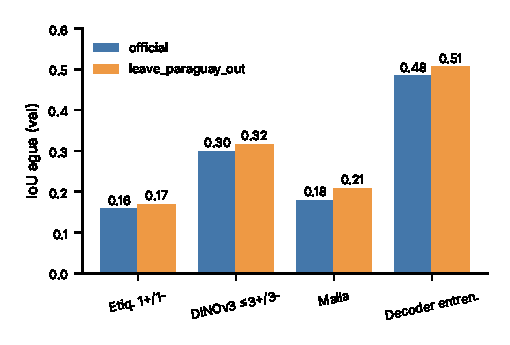
\includegraphics[width=\columnwidth]{fig_iou.pdf}\caption{IoU de agua en validaci\'on por fila (mismos datos que la tabla de resultados). Las filas no son todas comparables entre s\'i (ver texto).}\end{figure}
\textbf{Puntos simulados vs.\ autom\'aticos (decoder congelado).} Los puntos autom\'aticos duplican el IoU en ambos reg\'imenes, a costa de menos recall y m\'as precisi\'on. \emph{Salvedad que afecta la interpretaci\'on:} los puntos de etiqueta son 1+/1$-$ por componente real, los autom\'aticos hasta 3+/3$-$ por componente predicho (presupuestos reales 1\,204+/2\,055$-$ en official). No es una comparaci\'on con presupuesto igualado. La comparaci\'on pareada (referencia asistida 3+/3$-$, barridos de $k$) est\'a implementada en la etapa~7 pero \textbf{no se ejecut\'o}.\\
\begin{figure}[h]\centering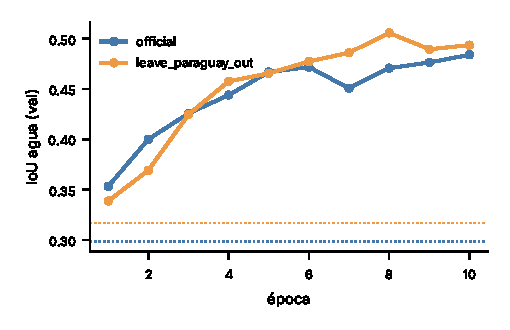
\includegraphics[width=\columnwidth]{fig_curvas.pdf}\caption{IoU de validaci\'on por \'epoca del decoder entrenado (etapa 6); las l\'ineas punteadas son la etapa 5 congelada.}\end{figure}
\begin{table}[h]\centering\footnotesize\caption{Etapa 6: m\'etricas de validaci\'on por \'epoca (de \texttt{curves.json}).}
\begin{tabular}{@{}rrrrr@{}}\toprule
\'Ep. & IoU off. & Dice off. & IoU excl. & Dice excl.\\\midrule
1 & 0.353 & 0.522 & 0.339 & 0.506\\
2 & 0.400 & 0.572 & 0.369 & 0.539\\
3 & 0.426 & 0.597 & 0.425 & 0.596\\
4 & 0.444 & 0.615 & 0.458 & 0.628\\
5 & 0.467 & 0.637 & 0.466 & 0.635\\
6 & 0.472 & 0.641 & 0.477 & 0.646\\
7 & 0.451 & 0.621 & 0.486 & 0.654\\
8 & 0.471 & 0.640 & 0.506 & 0.672\\
9 & 0.476 & 0.645 & 0.490 & 0.657\\
10 & 0.484 & 0.652 & 0.494 & 0.661\\
\bottomrule\end{tabular}\end{table}
\textbf{Congelado vs.\ ajustado.} Ajustar el decoder suma +18.5 pp (official) y +18.9 pp (excluido) respecto a la etapa 5, con una semilla; la mejor \'epoca y el umbral se eligieron en la misma validaci\'on. Es un efecto del decoder, no del prompt. En la intervenci\'on preliminar E2 (40 chips, puntos simulados, semilla 42) el IoU pas\'o de 0.170 a 0.308 en la \'epoca 1 y cay\'o a 0.150 en la \'epoca 4: el ajuste es inestable.\\
\textbf{Transferencia.} \emph{No evaluada.} La diferencia entre reg\'imenes ocurre en poblaciones de validaci\'on distintas y no prueba transferencia geogr\'afica.

\section{An\'alisis de fallos y limitaciones}
\begin{table}[h]\centering\footnotesize\caption{Cobertura de prompts (etapas 5--6, evidencia del repositorio).}
\begin{tabular}{@{}p{3.3cm}rr@{}}\toprule
& official & excluido\\\midrule
Chips val con prompts & 61/89 & 51/75\\
Chips val sin componentes (etapa 5) & 28/89 & 24/75\\
Train contribuyentes (etapa 6) & 161/252 & 139/213\\
Train sin componentes & 90 & 74\\\bottomrule
\end{tabular}\end{table}

\emph{Observado:} la mediana de IoU por chip con puntos autom\'aticos es baja (0.113/0.140) y la malla alcanza mediana 0; el decoder entrenado tiene cobertura parcial (61/89 chips de validaci\'on con prompts en official, el resto queda vac\'io); el r\'egimen excluido decae tras la \'epoca 8 (0.490, 0.494 en \'ep.~9--10). \emph{Hip\'otesis, no verificadas:} sombras, nubes o terreno oscuro como falsos positivos; el umbral alto de la sonda como causa de chips vac\'ios. No se revisaron ejemplos visuales en esta entrega. Limitaciones: una sola semilla, validaci\'on reutilizada para seleccionar, sin reservados, sin IC, solo SAM tiny y etapas 7--9 del plan inicial sin ejecutar.

\section{Procedimiento de reproducci\'on}
Las cifras de este informe se regeneran sin GPU con \texttt{python scripts/e3\_collect\_results.py}, que lee los JSON y el ZIP de evidencia del repositorio. Reejecutar los experimentos requiere Colab con GPU, los secretos de Hugging Face (\texttt{HF\_TOKEN}, no versionado) y acceso aprobado al modelo DINOv3 gated; los notebooks 05--07 contienen las celdas en orden (preparar, reiniciar el entorno y recuperar). Las pruebas locales (111 casos, sin modelos) verifican contratos de c\'odigo, no resultados cient\'ificos.

\section{Trabajo pendiente y reproducci\'on}
\textbf{Requisito pendiente:} (i) ejecutar en Colab la etapa~7 (A1--A3) y cerrar la comparaci\'on pareada; (ii) tras fijar la configuraci\'on en validaci\'on, evaluar transferencia con Bolivia y/o Paraguay reservado; (iii) incorporar la retroalimentaci\'on del workshop (18--20 nov), \textbf{pendiente de confirmaci\'on}. \textbf{Limitaci\'on:} una semilla, sin intervalos de confianza. \textbf{Mejora opcional:} an\'alisis visual de ejemplos de mejora y fallo, y SAM de mayor tama\~no. Las cifras se regeneran con \texttt{python scripts/e3\_collect\_results.py}; las etapas 5 y 6 las ejecut\'o R.~Ch\'avez en Colab T4 (evidencia en \texttt{docs/project/evidence/}), y la base E2 es trabajo conjunto ya publicado.

\section{Registro de decisiones y uso de IA}
El cuaderno de decisiones (\texttt{docs/project/cuaderno\_decisiones.md}) registra, para cada etapa, la hip\'otesis previa, la justificaci\'on, la configuraci\'on, las semillas, los resultados y los fallos. Semillas: 42 en E2; las etapas 5--6 usan las semillas fijadas en sus configuraciones (\texttt{configs/}). Fallos documentados: una descarga da\~nada del paquete de la etapa~5 (1\,067 entradas ilegibles) sustituida y re-auditada; la sonda con C=1 balanceada no convergi\'o y se excluy\'o por criterio previo. Asistencia de IA: implementaci\'on y auditor\'ia en CPU (Codex y Claude) sin ejecutar modelos; la ejecuci\'on en Colab la hicieron los integrantes. Los resultados se leen contra las salidas originales y no se han interpretado como evidencia de generalizaci\'on.

\section{Conclusiones}
Con decoder congelado, los prompts DINOv3 superan a 1+/1$-$ desde etiquetas en validaci\'on (0.299 vs.\ 0.158), pero el contraste no est\'a igualado en presupuesto. Entrenar el decoder es el mayor efecto observado (+18.5 pp). La pregunta de investigaci\'on queda respondida de forma \emph{descriptiva}; la respuesta controlada y la transferencia siguen pendientes (etapas 7--8).

\section{Intervenci\'on E2 previa}
\begin{table}[h]\centering\footnotesize\caption{E2: 40 chips de validaci\'on, puntos simulados, semilla 42, official.}
\begin{tabular}{@{}lrrrr@{}}\toprule
Brazo & IoU & Prec. & Rec. & Dice\\\midrule
Congelado & .170 & .171 & .964 & .291\\
Ajustado, mejor \'ep.~1 & .308 & .399 & .575 & .471\\\bottomrule
\end{tabular}\end{table}
La mejora de la mejor \'epoca proviene de menos falsos positivos (precisi\'on $.171\to.399$) a costa de recall ($.964\to.575$); la \'ultima \'epoca (IoU .150) muestra que el criterio de parada importa. Este resultado usa un subconjunto de 40 chips y no es comparable de forma directa con las 89 im\'agenes de las etapas 5--6.

\section{Estado de la demo, licencias y reproducibilidad}
La demo (Gradio) tiene pruebas locales de interfaz; \textbf{la carga de pesos reales y la inferencia punta a punta no se verificaron en esta entrega} (sin GPU ni acceso a Hugging Face desde el entorno de trabajo). Licencias consultadas: SAM~2.1, Apache-2.0 (tarjeta del modelo); DINOv3, licencia propia de Meta (redistribuci\'on bajo el mismo acuerdo, aviso ``Built with DINOv3'', restricciones de uso) \cite{dinov3license}; Sen1Floods11: la p\'agina del art\'iculo no indica licencia y la aclaraci\'on del repositorio sigue \textbf{pendiente}. Pesos, datos y checkpoints no se versionan. Asistencia de IA: registrada en el cuaderno de decisiones.

\begin{thebibliography}{9}\footnotesize
\bibitem{ravi2024sam2} N.~Ravi et al., ``SAM 2: Segment Anything in Images and Videos,'' arXiv:2408.00714, 2024.
\bibitem{simeoni2025dinov3} O.~Sim\'eoni et al., ``DINOv3,'' arXiv:2508.10104, 2025 (referencia a verificar contra el art\'iculo).
\bibitem{dinov3license} Meta AI, DINOv3 License, ai.meta.com/resources/models-and-libraries/dinov3-license.
\bibitem{bonafilia2020sen1floods11} D.~Bonafilia, B.~Tellman, T.~Anderson, E.~Issenberg, ``Sen1Floods11,'' CVPR Workshops, pp.~210--211, 2020.
\end{thebibliography}
\end{document}
